\subsection{Architettura backend}

\subsubsection{Descrizione generale} 
L’architettura del backend adotta lo stile modulare fornito da NestJS, basandosi su una suddivisione in moduli indipendenti, ciascuno responsabile di un sottoinsieme specifico delle funzionalità dell’applicazione. Ogni modulo è organizzato secondo un approccio a layer, comprendente controller, servizi e provider, favorendo la separazione delle responsabilità (Separation of Concerns).\\
Il ruolo principale del backend è quello di fungere da mediatore tra diverse fonti di dati esterne (principalmente API REST), aggregando e trasformando le informazioni ricevute in un formato uniforme e coerente. I dati vengono quindi resi disponibili tramite endpoint REST standardizzati. Le sorgenti dati sono incapsulate all’interno di componenti chiamati \textit{fetcher}, ognuno specializzato nell’interfacciamento con un’API specifica, e aderenti a una comune interfaccia astratta. Questo approccio garantisce estensibilità e flessibilità nella gestione di nuove fonti in futuro.

\subsubsection{Diagramma delle classi}
\begin{figure}[H]
    \begin{center}
        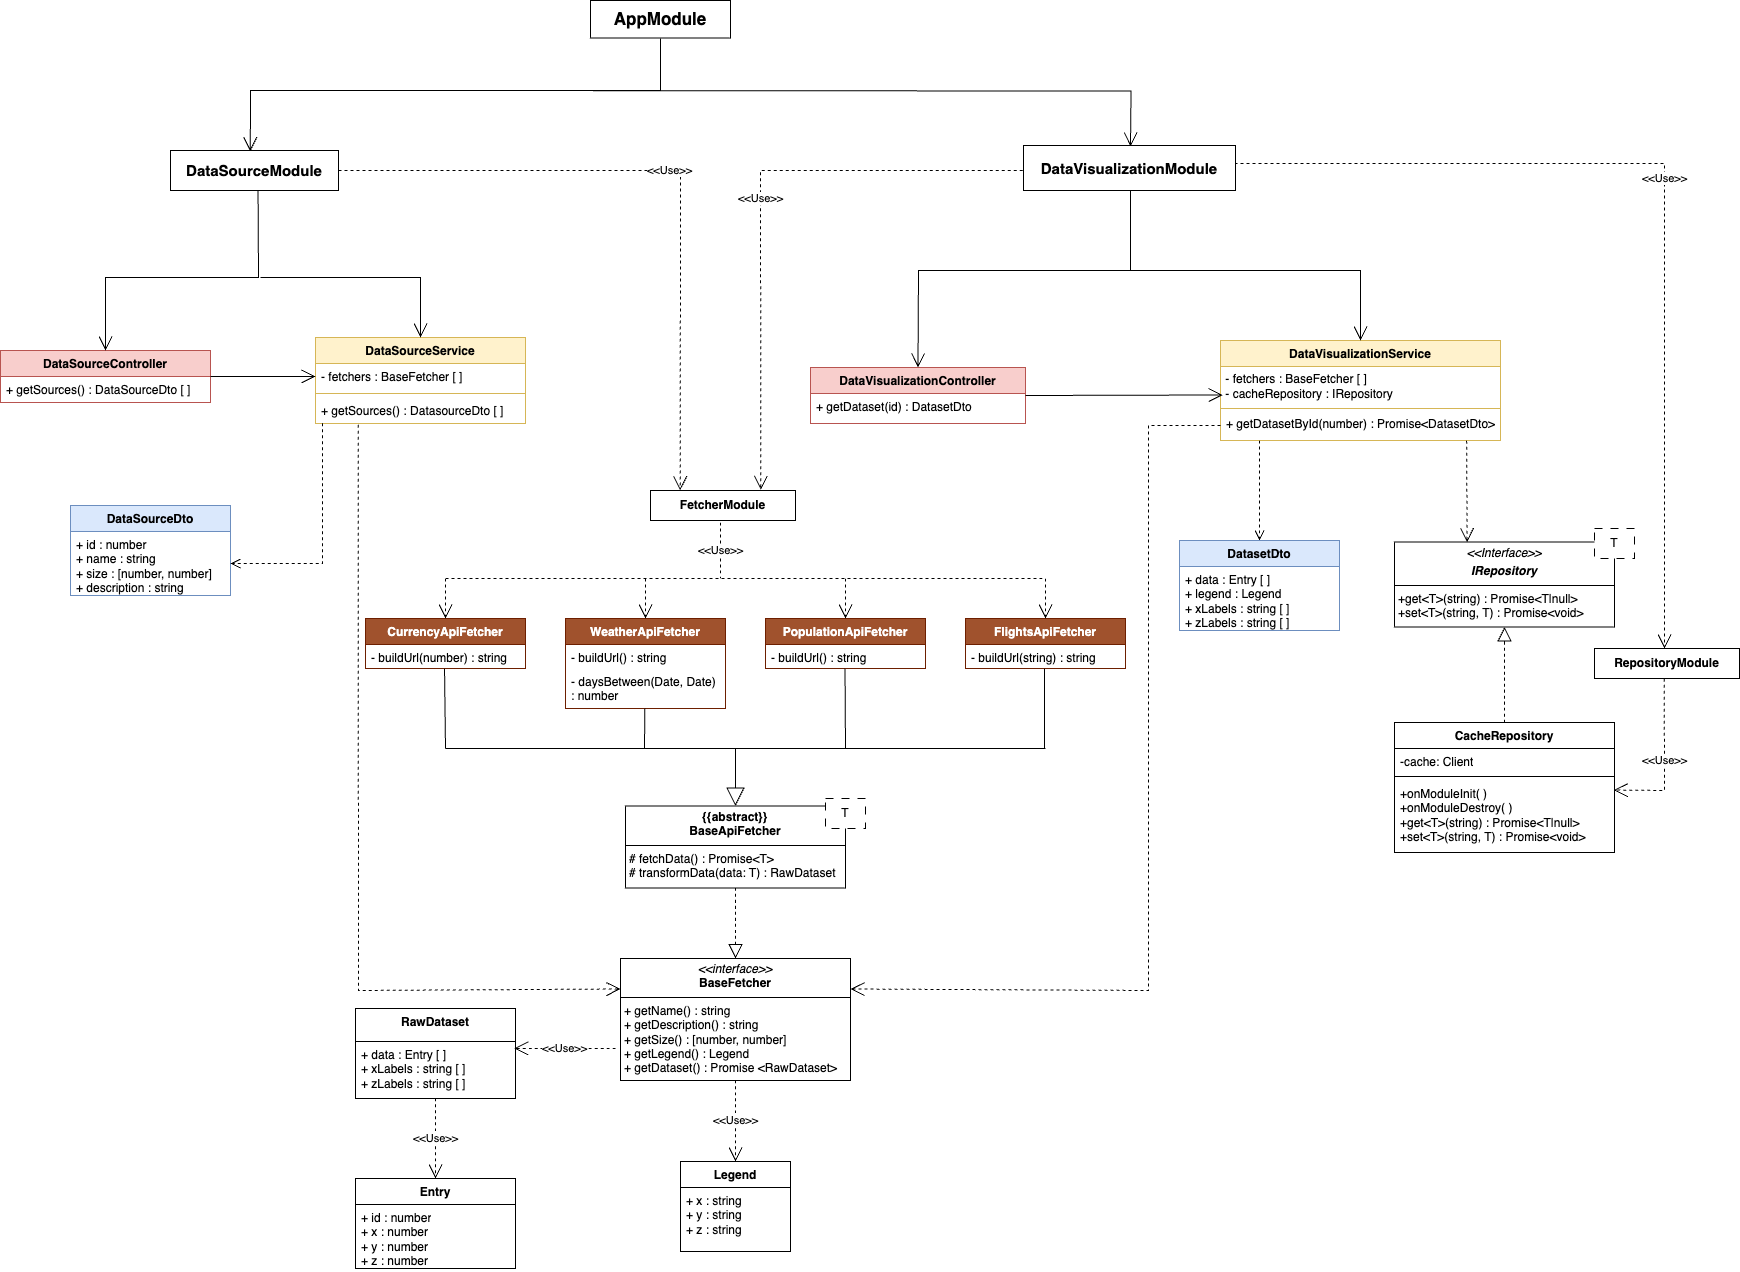
\includegraphics[scale = 0.29]{template/images/uml_back/BackendUML.png}
        \caption{Diagramma delle classi del backend}
    \end{center}     
    
\end{figure}

\subsubsection{Moduli}

L’architettura del sistema si articola in una serie di moduli specializzati, ciascuno dei quali si occupa di una specifica funzionalità o ambito logico dell’applicazione. Questa organizzazione facilita l’indipendenza tra componenti, promuove il riuso del codice e permette di mantenere alta la qualità progettuale anche in presenza di modifiche o estensioni future.\\
Ogni modulo interagisce con il resto del sistema attraverso interfacce ben definite, in modo da mantenere una chiara separazione tra le componenti. Questo approccio, ispirato alla programmazione modulare, favorisce l’estensibilità del progetto e semplifica le attività di test.\\
In NestJS, ogni modulo è una classe annotata con un decoratore \texttt{@Module()} che organizza logicamente i componenti dell’applicazione, come controller e servizi. L’integrazione tra moduli avviene tramite il sistema di imports ed exports, che consente di condividere funzionalità in modo esplicito e controllato.

\paragraph{AppModule}

\begin{figure}[H] 
    \centering
    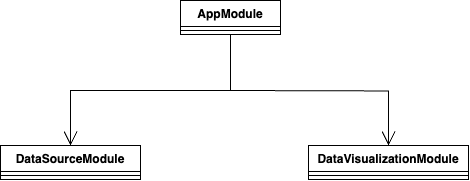
\includegraphics[scale = 0.6]{template/images/uml_back/AppModule.png}
    \caption{AppModule}
\end{figure}

L'AppModule rappresenta il punto di ingresso dell'applicazione. Il suo compito principale è orchestrare i moduli principali, separando chiaramente la logica applicativa dalle funzionalità di supporto. Questo modulo carica e configura i moduli principali, come \texttt{DataSourceModule} e \texttt{DataVisualizationModule}.

\paragraph{Moduli principali}
I moduli principali contengono la logica fondamentale dell'applicazione e sono responsabili della gestione e visualizzazione dei dati. I principali moduli dell'applicazione sono i seguenti:

\subparagraph{DataSourceModule}: 

\begin{figure}[H] 
    \centering
    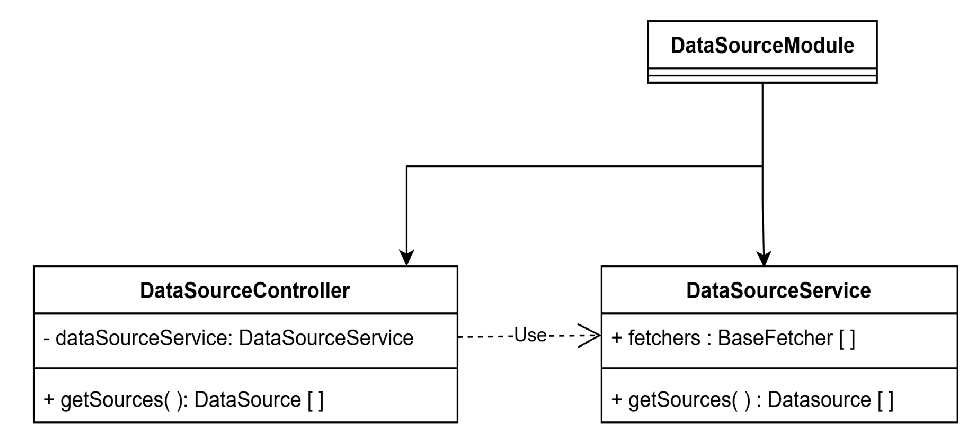
\includegraphics[scale = 0.4]{template/images/uml_back/DataSourceModule.png}
    \caption{DataSourceModule}
\end{figure}

Il \texttt{DataSourceModule} è responsabile della gestione delle metainformazioni relative alle fonti di dati disponibili nel sistema. Questo modulo incapsula la logica necessaria per raccogliere, organizzare e fornire informazioni descrittive sui dataset che l'applicazione può visualizzare.\\

\textbf{Responsabilità:}
\begin{itemize}
    \item Fornire un catalogo completo delle fonti dati disponibili
    \item Recuperare metadati descrittivi per ciascuna fonte (nome, dimensione, descrizione)
    \item Esporre queste informazioni attraverso endpoint REST standardizzati
    \item Organizzare i metadati in strutture DTO coerenti per il consumo da parte del frontend
\end{itemize}

\textbf{Componenti:}
\begin{itemize}
    \item \texttt{DataSourceController}: Espone l'endpoint HTTP \texttt{GET /data-source} che restituisce la lista completa delle fonti dati disponibili. Gestisce le richieste in arrivo, le instrada al servizio appropriato e serializza le risposte.
    
    \item \texttt{DataSourceService}: Implementa la logica di business per la raccolta dei metadati. Si interfaccia con i \texttt{fetcher} disponibili tramite l'interfaccia \texttt{BaseFetcher}, interrogando ciascuno per ottenere le informazioni descrittive necessarie. Questo servizio è responsabile della trasformazione dei dati grezzi in oggetti \texttt{DataSourceDto} ben strutturati.
    
    \item \texttt{DataSourceDto}: Definisce la struttura dei dati trasferiti dal backend al frontend. Include:
    \begin{itemize}
        \item \texttt{id}: Identificatore univoco della fonte dati
        \item \texttt{name}: Nome descrittivo della fonte
        \item \texttt{size}: Dimensione approssimativa del dataset
        \item \texttt{description}: Descrizione dettagliata del contenuto e dell'utilità della fonte
    \end{itemize}
\end{itemize}

\textbf{Dipendenze:}
\begin{itemize}
    \item \texttt{FetcherModule}: Fornisce accesso all'array di \texttt{BaseFetcher} attraverso il token di iniezione \texttt{FETCHERS}. Questo permette al \texttt{DataSourceService} di iterare attraverso i fetcher disponibili e raccogliere i metadati necessari.
    
    \item \texttt{BaseFetcher}: Interfaccia che definisce il contratto che ogni fetcher deve rispettare, inclusi i metodi per ottenere metadati descrittivi come \texttt{getName()}, \texttt{getDescription()} e \texttt{getSize()}.
\end{itemize}

\subparagraph{DataVisualizationModule}:

\begin{figure}[H] 
    \centering
    \includegraphics[scale = 0.5]{template/images/uml_back/DataVisModule.png}
    \caption{DataVisualizationModule}
\end{figure}

Il \texttt{DataVisualizationModule} gestisce la logica di recupero e formattazione dei dataset per la visualizzazione. Questo modulo si integra con il frontend permettendo di selezionare e visualizzare i dati provenienti dalle diverse fonti disponibili.\\

\textbf{Responsabilità:}
\begin{itemize}
    \item Recuperare il dataset completo dal fetcher selezionato dall'utente tramite un ID specifico
    \item Implementare una strategia di caching per velocizzare il caricamento dei dati già richiesti in precedenza
    \item Esporre un endpoint REST standardizzato per l'accesso ai dataset formattati
\end{itemize}

\textbf{Componenti:}
\begin{itemize}
    \item \texttt{DataVisualizationController}: Espone l'endpoint HTTP \texttt{GET /data-visualization/:id} che accetta l'ID numerico di un dataset e restituisce il dataset completo corrispondente.
    \item \texttt{DataVisualizationService}: Implementa la logica per il recupero del dataset richiesto. Il servizio verifica la validità dell'ID, controlla la disponibilità dei dati nella cache e, se necessario, utilizza il fetcher appropriato per ottenere i dati dalla fonte esterna.
    \item \texttt{DatasetDto}: Definisce la struttura dei dati restituiti al frontend, composta da:
    \begin{itemize}
        \item \texttt{rawData}: Dati grezzi recuperati dalla fonte esterna
        \item \texttt{legend}: Informazioni sulla legenda per la corretta visualizzazione del dataset
    \end{itemize}
\end{itemize}

\textbf{Dipendenze:}
\begin{itemize}
    \item \texttt{FetcherModule}: Fornisce accesso all'array di \texttt{BaseFetcher} attraverso il token di iniezione \texttt{FETCHERS}.
    \item \texttt{RepositoryModule}: Fornisce accesso all'interfaccia \texttt{IRepository} per la gestione della cache.    
    \item \texttt{BaseFetcher}: Interfaccia che definisce i metodi:
    \begin{itemize}
        \item \texttt{getDataset()}: Recupera i dati grezzi dalla fonte esterna
        \item \texttt{getLegend()}: Recupera le informazioni di legenda
    \end{itemize}
    
    \item \texttt{IRepository}: Interfaccia per la gestione della cache con operazioni di base:
    \begin{itemize}
        \item \texttt{get(key: string)}: Recupera un valore dalla cache
        \item \texttt{set(key: string, value: T)}: Memorizza un valore nella cache
    \end{itemize}
\end{itemize}


\paragraph{Moduli di supporto}
I moduli di supporto forniscono funzionalità tecniche o infrastrutturali necessarie al funzionamento dell’applicazione, ma non contengono logica di dominio.
Essi vengono progettati per essere riutilizzabili, indipendenti e incapsulati, e vengono esportati verso i moduli principali che ne fanno uso.
Esempi in questo progetto includono il \texttt{FetcherModule} e il \texttt{RepositoryModule}, che offrono rispettivamente l'accesso ai dati esterni e la logica di persistenza tramite cache.


\subparagraph{FetcherModule}:

\begin{figure}[H] 
    \centering
    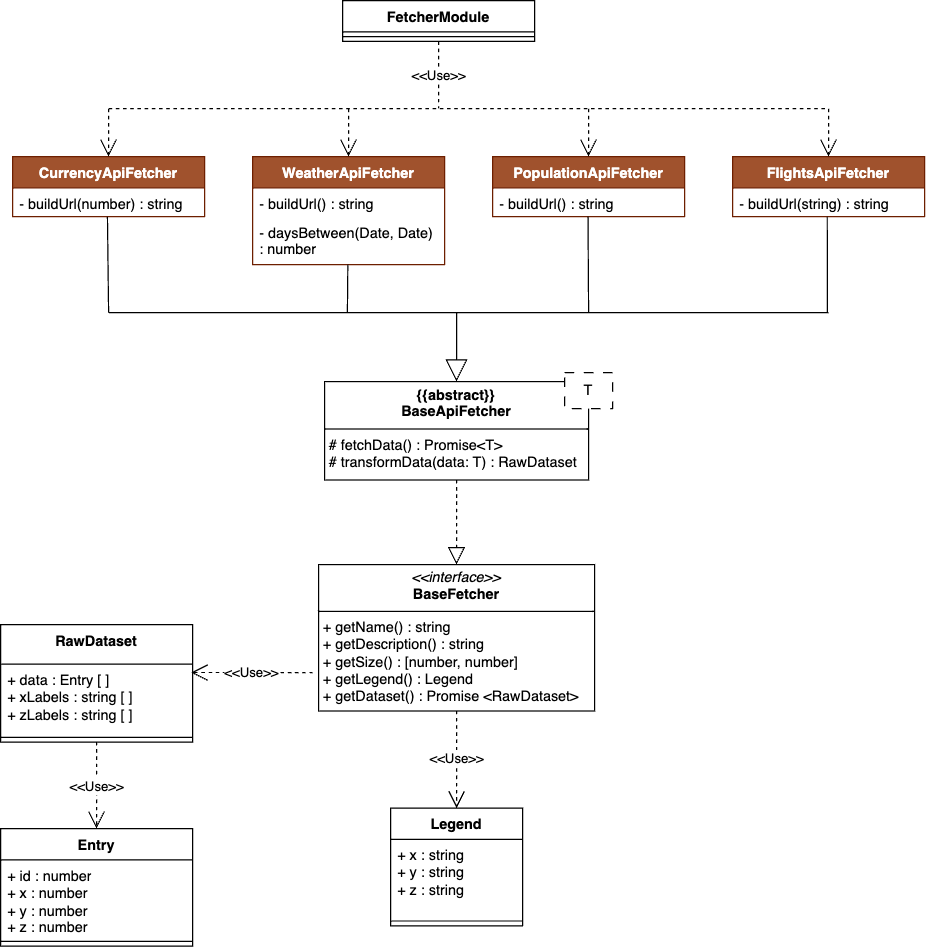
\includegraphics[scale = 0.4]{template/images/uml_back/FetcherModule.png}
    \caption{FetcherModule}
\end{figure}

Il \texttt{FetcherModule} incapsula tutti i componenti responsabili del recupero dei dati da fonti esterne, come API. Non contiene logica di business, ma espone un'interfaccia modulare e coerente per l’accesso ai dati, facilitando l’estensione e la manutenibilità del sistema.\\

\textbf{Responsabilità:}
\begin{itemize}
    \item Registrare e gestire i diversi \texttt{fetcher} che implementano l’interfaccia \texttt{BaseFetcher}.
    \item Fornire un punto di accesso centralizzato e modulare alle fonti dati esterne.
\end{itemize}

\textbf{Struttura del modulo:}
\begin{itemize}
    \item \texttt{BaseFetcher}: interfaccia che definisce il contratto da rispettare per ogni \texttt{fetcher}.
    \item \texttt{BaseApiFetcher}: classe astratta che offre una base comune per tutti i \texttt{fetcher} basati su API REST.
\end{itemize}

\textbf{Fetcher concreti:}
\begin{itemize}
    \item \texttt{WeatherApiFetcher}: recupera informazioni sulla temperatura media oraria per alcune grandi città europee, dal 01/01/2025 al 31/03/2025.
    \item \texttt{PopulationApiFetcher}: ottiene dataset contenente la popolazione totale di alcuni paesi dal 1974 al 2023.
    \item \texttt{FlightsApiFetcher}: fornisce il numero di partenze aeree da alcuni aeroporti internazionali nelle diverse fasce orarie in una giornata.
    \item \texttt{CurrencyApiFetcher}: restituisce tassi di cambio rispetto all'Euro campionati all'inizio di ogni anno dal 2005 al 2025.
\end{itemize}

\textbf{Integrazione con altri moduli:} \\
Il \texttt{FetcherModule} esporta il provider \texttt{FETCHERS}, che aggrega le istanze concrete dei \texttt{fetcher}. Questo consente agli altri moduli dell’applicazione di iniettarli facilmente, seguendo i principi dell’inversione delle dipendenze.

\subparagraph{RepositoryModule}:

\begin{figure}[H] 
    \centering
    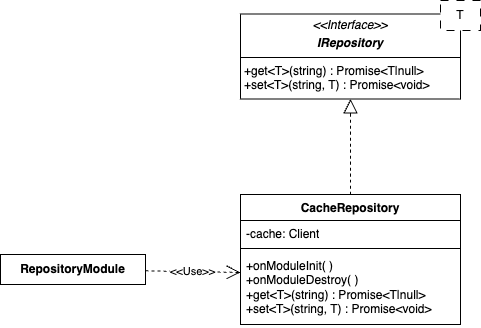
\includegraphics[scale = 0.5]{template/images/uml_back/RepositoryModule.png}
    \caption{RepositoryModule}
\end{figure}

Il \texttt{RepositoryModule} si occupa della persistenza temporanea dei dati applicativi, fornendo un’interfaccia coerente per la memorizzazione e il recupero di dati in cache. Questo modulo utilizza \texttt{Memcached}, tramite il client \texttt{memjs}, come sistema di caching.\\

\textbf{Responsabilità:}
\begin{itemize}
    \item Fornire un meccanismo centrale per l’accesso ai dati temporanei.
    \item Isolare l’implementazione della cache dai consumatori, attraverso l’uso di un’interfaccia.
\end{itemize}

\textbf{Struttura del modulo:}
\begin{itemize}
    \item \texttt{IRepository<T>}: interfaccia generica che definisce le operazioni base di salvataggio e lettura.
    \item \texttt{CacheRepository}: implementazione concreta che gestisce la connessione a Memcached e fornisce serializzazione JSON per i dati.
\end{itemize}

\textbf{Funzionalità del CacheRepository:}
\begin{itemize}
    \item Si connette al server Memcached all’avvio del modulo (\texttt{onModuleInit}).
    \item Chiude la connessione in fase di distruzione del modulo (\texttt{onModuleDestroy}).
    \item Metodo \texttt{get(key: string)}: recupera e deserializza il valore associato alla chiave specificata.
    \item Metodo \texttt{set(key: string, value: T)}: serializza e salva un valore con una chiave e un TTL predefinito.
    \item Gestione robusta degli errori: i fallimenti di cache non interrompono il flusso del programma.
\end{itemize}

\textbf{Integrazione con altri moduli:} \\
Il modulo esporta l’interfaccia \texttt{IRepository} attraverso un provider personalizzato, iniettando dietro l’implementazione concreta \texttt{CacheRepository}. Questo approccio permette, ad esempio al \texttt{DataVisualizationService}, di interagire con la cache senza dipendere direttamente dall’implementazione, favorendo un basso accoppiamento e una maggiore flessibilità.



\subsection{Pattern architetturale e Design pattern}

\subsubsection{Architettura Modulare (Modular Architecture)}
L’architettura del backend è progettata seguendo un approccio modulare, in cui ogni modulo rappresenta un'unità funzionale autonoma. Ciò consente di isolare le responsabilità, facilitando la manutenibilità e l'estensibilità del sistema. Ogni modulo è progettato per essere riutilizzabile e facilmente testabile, seguendo i principi della separazione delle preoccupazioni.

\subsubsection{Architettura a Strati (Layered Architecture)}
All'interno di ogni modulo, l'architettura a strati separa le diverse responsabilità: controller per la gestione delle richieste, servizi per la logica applicativa, e possibilmente DTO per la definizione dei dati scambiati. Questa separazione migliora la manutenibilità e la testabilità dell'applicazione.

\begin{itemize}  
  \item \textbf{Controller (Presentation Layer):} Gestiscono le richieste in ingresso (es. HTTP) e costituiscono l'interfaccia tra il client e l'applicazione. Utilizzano decoratori come \texttt{@Controller} e \texttt{@Get} per definire le rotte e delegare la logica ai servizi sottostanti. Non contengono logica di business, ma si occupano di validare i dati tramite i DTO e restituire le risposte.
  
  \item \textbf{Service (Application Layer):} Implementano la logica applicativa e orchestrano le operazioni necessarie per soddisfare le richieste. I servizi sono iniettati nei controller tramite il pattern di Dependency Injection e gestiscono la business logic dell'applicazione, interagendo con repository, fetcher, o database.
  
  \item \textbf{DTO (Data Transfer Object):} Definiscono i dati scambiati tra client e server, specificando le proprietà che devono essere validate e mappate. I DTO aiutano a garantire la coerenza dei dati e a documentare le API.
\end{itemize}

\subsubsection{Design Pattern Utilizzati}

In NestJS, abbiamo sfruttato diversi design pattern per semplificare la struttura e migliorare la manutenibilità del codice:

\begin{itemize}
  \item \textbf{Dependency Injection (DI):} Il pattern DI è utilizzato da NestJS per gestire le dipendenze tra i componenti. Grazie al decoratore \texttt{@Injectable()}, i servizi possono essere iniettati in altri servizi o controller. Questo approccio riduce il coupling e migliora la testabilità del sistema, evitando la creazione manuale delle istanze.

  \item \textbf{Decorator Pattern (con \texttt{@Controller} e \texttt{@Get}):} NestJS fa ampio uso del pattern decoratore, che permette di aggiungere comportamenti specifici ai componenti senza modificarne il codice. Il decoratore \texttt{@Controller} viene utilizzato per definire un controller, mentre \texttt{@Get} è impiegato per associare una rotta HTTP GET a un metodo del controller. Questi decoratori semplificano la gestione delle rotte e delle richieste HTTP.
  
  \item \textbf{Singleton:} Il pattern Singleton è applicato a livello di servizio, in quanto NestJS gestisce i provider come istanze uniche durante il ciclo di vita dell'applicazione. I servizi sono quindi condivisi tra i vari componenti, ottimizzando le risorse e riducendo il carico di creazione di nuove istanze.

  \item \textbf{Repository Pattern:} Utilizzato per astrarre la logica di accesso ai dati dalla logica di business, il Repository Pattern consente di gestire l'interazione con le fonti dati (come database o cache) in modo centralizzato. I repository vengono iniettati nei servizi, permettendo una gestione più flessibile dei dati.
\end{itemize}

